\chapter{Introduction}
\label{chapter_introduction}

Computer graphics are being used in more and more areas today to help with visualization of data, such as in big data and crowd simulation. However human body animation and cloth simulation have been two significant subjects of the field for a while. Although there are cases where the simulation results are incredibly life-like, the task is still nothing trivial. 

One of the most time-consuming stages of apparel shopping is trying the apparels on, which is not even possible in online stores. With the advances in augmented reality technologies, virtual fitting rooms are slowly taking their places in both real and virtual stores~\cite{Fitnect2012,Styku2013} to improve the quality of apparel trial experience while also making it faster. On the low-end of the spectrum, there are super positioned 2D images of the user and the apparel, without any animation. Advanced virtual fitting rooms on the other hand, show the apparel items either on the video of the user or on a virtual avatar, both scaled to reflect the user's body characteristics~\cite{FaceCake2013}. Some of them also employ physics-based garment simulation for a better fitting experience~\cite{Styku2013}.

This study is aimed to develop a novel virtual fitting room framework that provides all the basic features expected from such an application, along with enhancements in various aspects for higher realism. These enhancements include motion filtering, customized user scaling, and physics engine. Motion filtering process starts with temporal averaging of joint positions in order to overcome the high noise of the depth sensor. However, temporal averaging does not prove to be sufficient because unnatural movements take place due to limited recognition capabilities and self-occlusion. Customized joint angle filters, along with bone splitting to let limbs twist in a more natural way and footskate correction filters are implemented. The overall framework is shown in Figure~\ref{fig:overall}. 

\begin{figure}[htbp]
	\centerline{
	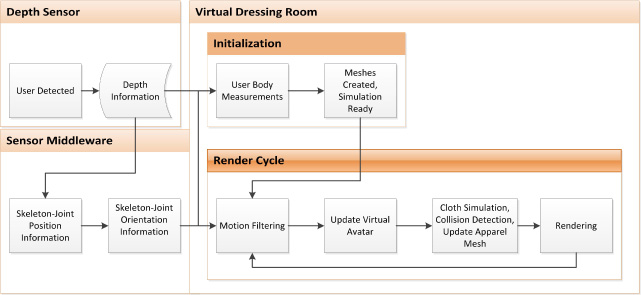
\includegraphics[width=1.0\textwidth]{./figures/overall.eps}
	}
	\caption{The overall virtual dressing framework}
	\label{fig:overall}
\end{figure}


The avatar utilizes a skeleton which conforms with the LOA 2 of H-ANIM 200x specification~\cite{HANIM}, although not all bones are used for animation because of the available data from depth sensor. The skeleton and mesh are modeled in Blender~\cite{Blender}, exported and used in binary format. The simulated apparel pieces are also modeled in Blender, although they are exported in Wavefront OBJ format in order to be parsed by the physics engine. They are binarized on-the-run to be used by the game engine. 

The cloth pieces to be fitted on the user's avatar must first be scaled accordingly. To this end, a body measurement process is implemented, which starts with depth map smoothing, in order to reduce the noise. Afterwards, the filtered depth map is utilize along with filtered user joints to measure a set of parameters, which are used in conjunction to estimate the body height and width. These parameters are averaged over time to minimize the error.

The physics engine utilizes collision spheres and capsules to perform collision detection. The correct sphere radii and positions are determined during body measurements. The virtual avatar is aligned with a set of invisible spheres and capsules are aligned with joints and limbs, which are updated in real time and used in collision detection. Cloth particles are also affected by gravity and inertia.


\section{Organization of the Thesis}

The thesis is organized as follows. Chapter~\ref{chapter_related_work}, we give related work on virtual fitting rooms and 
depth sensors. Chapter~\ref{chapter_3d_model} describes the human and cloth modeling for virtual fitting room. Chapter~\ref{chapter_animation} focuses on the animation techniques along with various optimizations for a realistic experience. Chapter~\ref{chapter_cloth_simulation} discusses the physics engine and cloth simulation process. Chapter~\ref{chapter_cloth_resizing} deals with the cloth resizing process for a customized fitting experience. The experiments, performance qualities and results are presented in~\ref{chapter_experiments}. Chapter~\ref{chapter_conclusion} outlines the thesis and shows the future direction of this research. Appendix~\ref{appendix_ogre_framework} describes the game engine which provides the boilerplate functions for our framework. Appendix~\ref{appendix_user_tracking} gives information about the depth sensor and its user tracking capabilities. A user interaction feature, depth-based hand tracking is explained in Appendix~\ref{appendix_hand_tracking}.
